% Substack header — 1100x220 PNG target
% Compile: pdflatex header.tex
% Convert: pdftocairo -png -scale-to-x 1100 -scale-to-y 220 header.pdf header
%
% Design: two horizontal lines of dots stream in from the left/right edges,
% then curl smoothly into a two-arm spiral at the center.
% The curve r(t) = rOuter * (rInner/rOuter)^t with phi(t) = thetamax * t^2
% has a horizontal tangent at t=0, so the spiral joins the straight line
% with no visible kink. Dots are placed at uniform arc length using
% decorations.markings. Dots stay at full size on the line, then shrink
% linearly from full size to zero across the spiral.

\documentclass[tikz,border=0pt]{standalone}
\usepackage{tikz}
\usetikzlibrary{decorations.markings}
\usepackage{xcolor}

% Palette
\definecolor{leftc}{HTML}{3F9580}     % green, nudged toward teal
\definecolor{rightc}{HTML}{D43A28}    % burnt orange, nudged toward red
\definecolor{bgc}{HTML}{FFF8E4}       % cream / parchment

\begin{document}
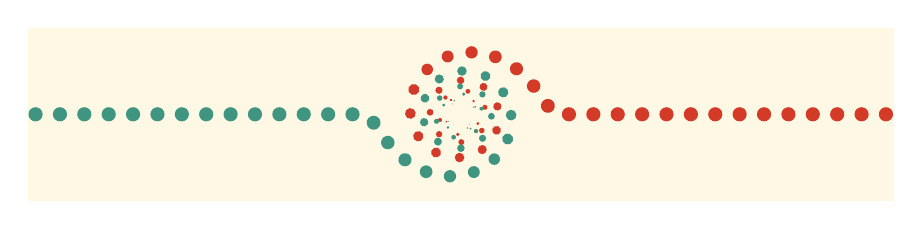
\begin{tikzpicture}[x=1cm,y=1cm]
  \useasboundingbox (-5.5,-1.1) rectangle (5.5,1.1);
  \fill[bgc] (-5.5,-1.1) rectangle (5.5,1.1);

  % ==========================================================
  %                     PARAMETERS
  % ==========================================================
  \def\rOuter{1.25}         % spiral outer radius (cm)  — bigger nucleus
  \def\rInner{0.15}         % spiral inner radius (cm)  — tight; dots fade before crowding
  \def\turnsTotal{5.0}      % more turns => more vertical reach & dots stay thick longer
  \def\canvasEdge{5.40}     % outermost x of the horizontal dot lines (cm)

  \def\Ndots{50}            % dots per arm
  \def\dotRad{0.09}         % full dot radius (cm) — line dots & first spiral dot

  % Spiral chirality:
  %   \leftYSign = +1  →  yin-yang (left arm mirrored across y-axis, opposite-winding)
  %   \leftYSign = -1  →  galaxy   (left arm rotated 180°, both arms same direction)
  \def\leftYSign{-1}

  % ==========================================================
  %                     DERIVED
  % ==========================================================
  \pgfmathsetmacro{\thetamaxDeg}{360*\turnsTotal}
  \pgfmathsetmacro{\thetaMaxRad}{2*pi*\turnsTotal}
  \pgfmathsetmacro{\lnratio}{ln(\rInner/\rOuter)}
  \pgfmathsetmacro{\stepsize}{1/(\Ndots-1)}
  \pgfmathsetmacro{\lineLen}{\canvasEdge - \rOuter}

  % Numerically estimate the spiral arc length, so we know what fraction of the
  % whole path is the straight line. Used to gate the shrink in the mark code.
  \xdef\spiralLen{0}
  \foreach \kk in {1,...,50} {
    \pgfmathsetmacro{\tk}{(\kk-0.5)/50}
    \pgfmathsetmacro{\rk}{\rOuter*exp(\lnratio*\tk)}
    \pgfmathsetmacro{\dphi}{2*\thetaMaxRad*\tk}
    \pgfmathsetmacro{\dsdt}{\rk*sqrt(\lnratio*\lnratio + \dphi*\dphi)}
    \pgfmathsetmacro{\newLen}{\spiralLen + \dsdt/50}
    \xdef\spiralLen{\newLen}
  }
  \pgfmathsetmacro{\totalLen}{\lineLen + \spiralLen}
  \pgfmathsetmacro{\lineFrac}{\lineLen/\totalLen}

  % ==========================================================
  %                     RIGHT ARM (burnt orange-red)
  % ==========================================================
  \path[postaction={decorate}, decoration={
      markings,
      mark=between positions 0 and 1 step \stepsize with {
        \pgfmathsetmacro{\fracAlong}{\pgfdecoratedcompleteddistance/\pgfdecoratedpathlength}
        \pgfmathsetmacro{\ds}{\fracAlong<\lineFrac
          ? \dotRad
          : \dotRad*(1-(\fracAlong-\lineFrac)/(1-\lineFrac))}
        \fill[rightc] (0,0) circle (\ds cm);
      }
    }]
    (\canvasEdge,0) -- (\rOuter,0)
    plot[domain=0:1, samples=150, variable=\t]
      ({\rOuter*exp(\lnratio*\t)*cos(\thetamaxDeg*\t*\t)},
       {\rOuter*exp(\lnratio*\t)*sin(\thetamaxDeg*\t*\t)});

  % ==========================================================
  %                     LEFT ARM (green) — mirrored
  % ==========================================================
  \path[postaction={decorate}, decoration={
      markings,
      mark=between positions 0 and 1 step \stepsize with {
        \pgfmathsetmacro{\fracAlong}{\pgfdecoratedcompleteddistance/\pgfdecoratedpathlength}
        \pgfmathsetmacro{\ds}{\fracAlong<\lineFrac
          ? \dotRad
          : \dotRad*(1-(\fracAlong-\lineFrac)/(1-\lineFrac))}
        \fill[leftc] (0,0) circle (\ds cm);
      }
    }]
    (-\canvasEdge,0) -- (-\rOuter,0)
    plot[domain=0:1, samples=150, variable=\t]
      ({-\rOuter*exp(\lnratio*\t)*cos(\thetamaxDeg*\t*\t)},
       {\leftYSign*\rOuter*exp(\lnratio*\t)*sin(\thetamaxDeg*\t*\t)});

\end{tikzpicture}
\end{document}
